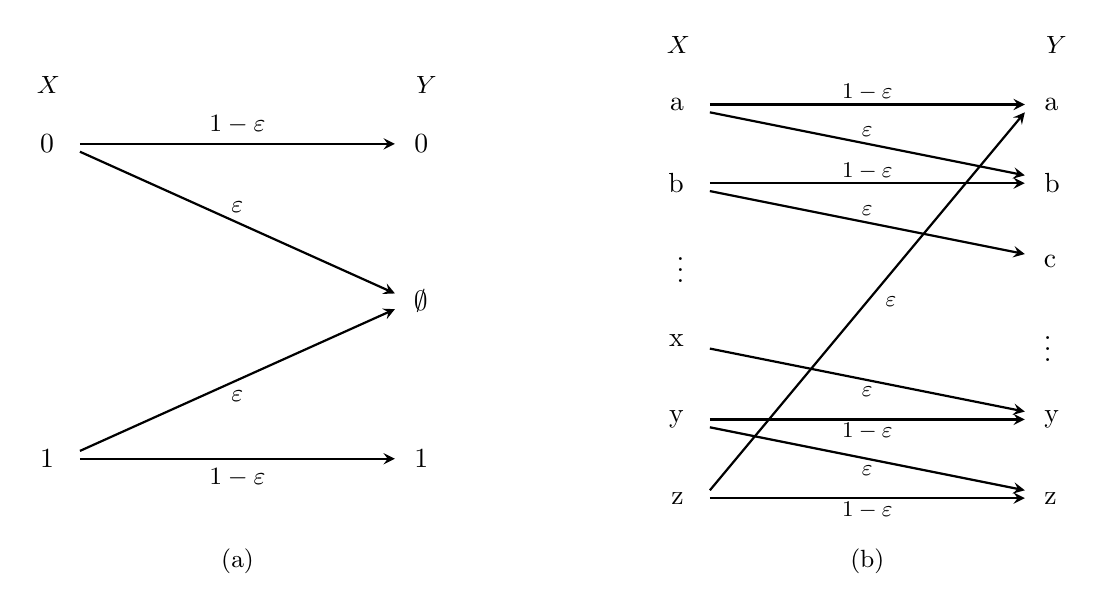
\begin{tikzpicture}
\shorthandoff{>}
%
% Canal borrador
\begin{scope}
\draw (-.4,2.75) node {\small $X$}; \draw (4.4,2.75) node {\small $Y$};
%
\draw[>=stealth,->,thick] (-.2,2) node[left]{0} (0,2) -- (4,2) node[right]{\ 0};
\draw (2,2) node[above]{\small $1-\varepsilon$};
%
\draw[>=stealth,->,thick] (-.2,-2) node[left]{1} (0,-2) -- (4,-2) node[right]{\ 1};
\draw (2,-2) node[below]{\small $1-\varepsilon$};
%
\draw[>=stealth,->,thick] (0,1.9)--(4,.1);
\draw (2,1.2) node{\small $\varepsilon$};
\draw[>=stealth,->,thick] (0,-1.9)--(4,-.1);
\draw (2,-1.2) node{\small $\varepsilon$};
\draw (4,0) node[right]{\ $\emptyset$};
%
\end{scope}
%
% Canal typewriter
\begin{scope}[xshift = 8cm]
\draw (-.4,3.25) node {\small $X$}; \draw (4.4,3.25) node {\small $Y$};
%
% lineas sin error
\draw[>=stealth,->,thick] (-.2,2.5) node[left]{a} (0,2.5) -- (4,2.5) node[right]{\ a};
\draw (2,2.65) node[scale=.9]{\small $1-\varepsilon$};
\draw[>=stealth,->,thick] (-.2,1.5) node[left]{b} (0,1.5) -- (4,1.5) node[right]{\ b};
\draw (2,1.65) node[scale=.9]{\small $1-\varepsilon$};
\draw (-.2,.5) node[left]{$\vdots$}; \draw (4,-.5) node[right]{\ $\vdots$};
\draw[>=stealth,->,thick] (-.2,-1.5) node[left]{y} (0,-1.5) -- (4,-1.5) node[right]{\ y};
\draw (2,-1.65) node[scale=.9]{\small $1-\varepsilon$};
\draw[>=stealth,->,thick] (-.2,-2.5) node[left]{z} (0,-2.5) -- (4,-2.5) node[right]{\ z};
\draw (2,-2.65) node[scale=.9]{\small $1-\varepsilon$};
%
% lineas con el error
\draw[>=stealth,->,thick] (0,2.4) -- (4,1.6);
\draw (2,2.15) node[scale=.9]{\small $\varepsilon$};
\draw[>=stealth,->,thick] (0,1.4) -- (4,.6); \draw (4,.5) node[right]{\ c};
\draw (2,1.15) node[scale=.9]{\small $\varepsilon$};
\draw[>=stealth,->,thick]  (-.2,-.5) node[left]{x} (0,-.6) -- (4,-1.4);
\draw (2,-1.15) node[scale=.9]{\small $\varepsilon$};
\draw[>=stealth,->,thick] (0,-1.6) -- (4,-2.4);
\draw (2,-2.15) node[scale=.9]{\small $\varepsilon$};
\draw[>=stealth,->,thick] (0,-2.4) -- (4,2.4);
\draw (2.3,0) node[scale=.9]{\small $\varepsilon$};
%
\end{scope}
\draw (2,-3.3) node{\small (a)};
\draw (10,-3.3) node{\small (b)};
\end{tikzpicture}
